

\title{HW3 For Applied Data Mining \\ STAT W 3026-4026 \\ Spring 2016 \\ Columbia University}
\author{
       Robin Lee  \\
               rcl2136\\
      QMSS MA}
\date{\today}

\documentclass[12pt]{article}

\makeatletter
\newcommand*{\rom}[1]{\expandafter\@slowromancap\romannumeral #1@}
\makeatother
\usepackage{amsthm,amsmath,graphicx,csquotes}
\usepackage[
         colorlinks=true,
         linkcolor=black,
         citecolor=black,
         urlcolor=black]
         {hyperref}  
         
\newtheorem{thm}{Theorem}
\newtheorem{defn}{Definition}
%\newtheorem{rem}{Remark}
%\newtheorem{lem}{Lemma}
\newtheorem{prop}{Property}

\setkeys{Gin}{width=0.8\textwidth}

\usepackage{Sweave}
\begin{document}
\Sconcordance{concordance:hw3.tex:hw3.Rnw:%
1 30 1 1 0 11 1 1 2 1 0 5 1 17 0 1 2 5 1 1 3 6 0 1 2 8 1 1 2 1 0 2 1 9 %
0 1 2 5 1 1 2 1 0 1 2 1 1 12 0 1 2 1 3 1 0 1 3 1 0 1 1 12 0 1 3 1 1 1 2 %
1 0 1 1 10 0 1 2 2 1 9 0 1 2 2 1 1 2 1 0 1 2 6 0 1 2 2 1 1 2 1 0 2 1 7 %
0 1 2 14 1 1 2 1 0 2 1 1 6 4 0 1 2 1 1 6 0 1 2 2 1 1 2 6 0 1 1 6 0 1 2 %
9 1 1 6 5 0 1 2 20 0 1 3 1 0 1 1 16 0 1 3 2 1 1 7 6 0 1 2 3 0 1 2 2 1 1 %
34 32 0 1 2 1 1 1 2 1 1 5 0 1 4 3 0 1 2 5 0 1 3 11 1 1 2 1 0 1 1 3 0 1 %
2 4 1 1 2 6 0 1 1 9 0 1 3 6 1 1 2 1 0 2 1 5 0 1 1 6 0 1 2 2 1}

\maketitle

%\begin{abstract}

%\end{abstract}

\section{Exercise 3.1}
The UC Irvine Machine Learning Repository6 contains a data set related to glass identification. The data consist of 214 glass samples labeled as one of seven class categories. There are nine predictors, including the refractive index and percentages of eight elements: Na, Mg, Al, Si, K, Ca, Ba, and Fe.

The data can be accessed via:
\begin{Schunk}
\begin{Sinput}
> library(ggplot2)
> library(GGally)
> library(dplyr)
> library(mlbench)
> data(Glass)
> glimpse(Glass)
\end{Sinput}
\begin{Soutput}
Observations: 214
Variables: 10
$ RI   (dbl) 1.52101, 1.51761, 1.51618, 1.51766, 1.51742, 1.51596, 1.51743,...
$ Na   (dbl) 13.64, 13.89, 13.53, 13.21, 13.27, 12.79, 13.30, 13.15, 14.04,...
$ Mg   (dbl) 4.49, 3.60, 3.55, 3.69, 3.62, 3.61, 3.60, 3.61, 3.58, 3.60, 3....
$ Al   (dbl) 1.10, 1.36, 1.54, 1.29, 1.24, 1.62, 1.14, 1.05, 1.37, 1.36, 1....
$ Si   (dbl) 71.78, 72.73, 72.99, 72.61, 73.08, 72.97, 73.09, 73.24, 72.08,...
$ K    (dbl) 0.06, 0.48, 0.39, 0.57, 0.55, 0.64, 0.58, 0.57, 0.56, 0.57, 0....
$ Ca   (dbl) 8.75, 7.83, 7.78, 8.22, 8.07, 8.07, 8.17, 8.24, 8.30, 8.40, 8....
$ Ba   (dbl) 0, 0, 0, 0, 0, 0, 0, 0, 0, 0, 0, 0, 0, 0, 0, 0, 0, 0, 0, 0, 0,...
$ Fe   (dbl) 0.00, 0.00, 0.00, 0.00, 0.00, 0.26, 0.00, 0.00, 0.00, 0.11, 0....
$ Type (fctr) 1, 1, 1, 1, 1, 1, 1, 1, 1, 1, 1, 1, 1, 1, 1, 1, 1, 1, 1, 1, 1...
\end{Soutput}
\end{Schunk}

\begin{itemize}
\item 
Using visualizations, explore the predictor variables to understand their distributions as well as the relationships between predictors.

My options are scatterplot matrix and histogram. Thus, I will use ggpairs in GGally package to get the plot. I also adjust the transparency to make scatter plots easier to read.
\begin{Schunk}
\begin{Sinput}
> ggpairs(Glass, columns= 1:9, 
+         mapping = ggplot2::aes(alpha = 0.2))
\end{Sinput}
\end{Schunk}
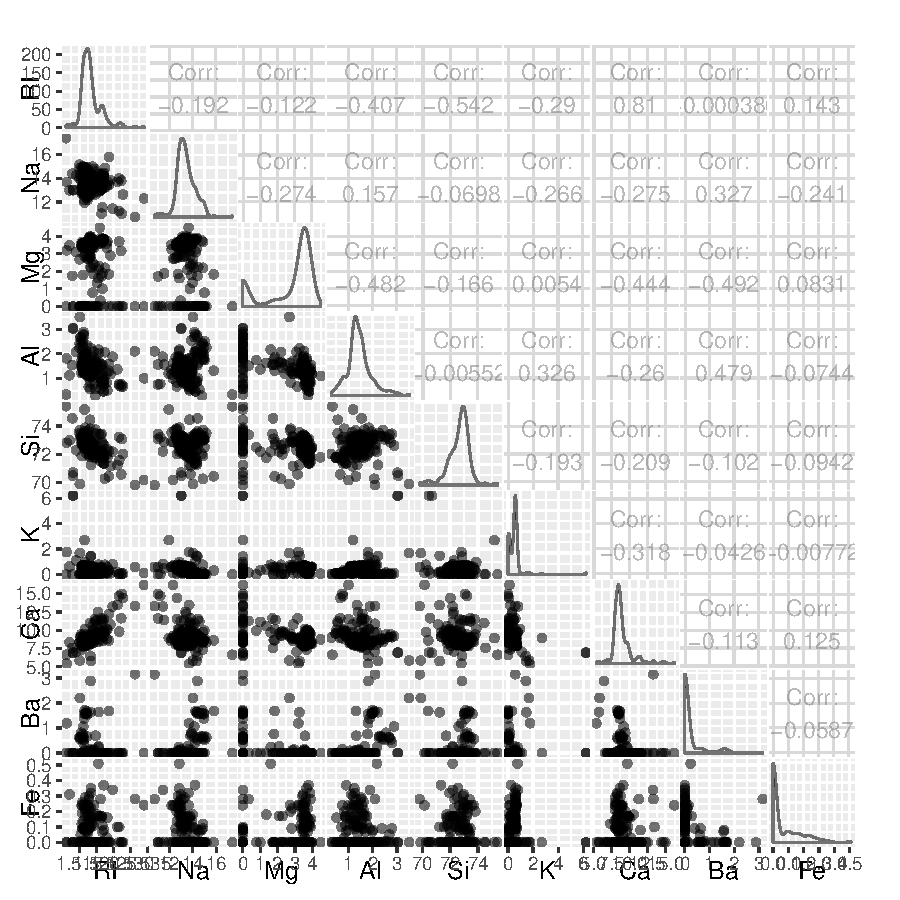
\includegraphics{hw3-002}

The only two predictors that have a correlation coefficient above 0.5 or below -0.5 are RI and Ca.

\item
Do there appear to be any outliers in the data? Are any predictors skewed?

Yes, from the histogras, Al, K, CA, Ba, and Fe are skewed to the right. Mg is skewed to the left and has a smaller peak on the left. There are some samples with high values in K, Ca and Ba.

I will calculate skewness to confirm.
\begin{Schunk}
\begin{Sinput}
> library(e1071)
> skewValues <- apply(Glass[,1:9], 2, skewness)
> skewValues
\end{Sinput}
\begin{Soutput}
        RI         Na         Mg         Al         Si          K         Ca 
 1.6027151  0.4478343 -1.1364523  0.8946104 -0.7202392  6.4600889  2.0184463 
        Ba         Fe 
 3.3686800  1.7298107 
\end{Soutput}
\end{Schunk}
The result is similar to what I got judging from the histograms.

\item
Are there any relevant transformations of one or more predictors that might improve the classification model?

Yes, for the skewed variables, I should transform the predictors. I will use Box-cox test to find out what transformation is needed.
\begin{Schunk}
\begin{Sinput}
> library(caret)
> boxcoxValues = preProcess(Glass[,-10],method = "BoxCox")
> boxcoxValues
\end{Sinput}
\begin{Soutput}
Created from 214 samples and 5 variables

Pre-processing:
  - Box-Cox transformation (5)
  - ignored (0)

Lambda estimates for Box-Cox transformation:
-2, -0.1, 0.5, 2, -1.1
\end{Soutput}
\begin{Sinput}
> BC = apply(Glass[,-10],2, BoxCoxTrans)
> # transform variables
> GlassBC = predict(boxcoxValues, Glass[,-10])
> # check if skewness is resolved
> skewValues2 <- apply(GlassBC, 2, skewness)
> skewValues2
\end{Sinput}
\begin{Soutput}
         RI          Na          Mg          Al          Si           K 
 1.56566039  0.03384644 -1.13645228  0.09105899 -0.65090568  6.46008890 
         Ca          Ba          Fe 
-0.19395573  3.36867997  1.72981071 
\end{Soutput}
\begin{Sinput}
> 
\end{Sinput}
\end{Schunk}
Some variables are not transformed with BoxCox. I will try to center and scale them!

\begin{Schunk}
\begin{Sinput}
> normalValues <- preProcess(Glass[,-10], method = c("center", "scale"))
> normalValues
\end{Sinput}
\begin{Soutput}
Created from 214 samples and 9 variables

Pre-processing:
  - centered (9)
  - ignored (0)
  - scaled (9)
\end{Soutput}
\begin{Sinput}
> GlassNormal = predict(normalValues, Glass[,-10])
> skewValues3 = apply(GlassNormal,2,skewness)
> skewValues3
\end{Sinput}
\begin{Soutput}
        RI         Na         Mg         Al         Si          K         Ca 
 1.6027151  0.4478343 -1.1364523  0.8946104 -0.7202392  6.4600889  2.0184463 
        Ba         Fe 
 3.3686800  1.7298107 
\end{Soutput}
\end{Schunk}
All 9 variables are scaled. But the skewness does not change. This makes sense actually. Normalizing the predictors does not change the shape.

I suspect some of these variables contain zeros. That's why log transformation is not possible.
\begin{Schunk}
\begin{Sinput}
> log = log(Glass[,c(3,6,8,9)])
> sum(Glass[,c(3,6,8,9)]==0)
\end{Sinput}
\begin{Soutput}
[1] 392
\end{Soutput}
\end{Schunk}
Yes, lots of zeros.

I will try squared root on these transformatioin
\begin{Schunk}
\begin{Sinput}
> sqrt = sqrt(Glass[,c(3,6,8,9)])
> skewValues4 = apply(sqrt,2,skewness)
> skewValues4
\end{Sinput}
\begin{Soutput}
        Mg          K         Ba         Fe 
-1.3460193  0.8590459  2.3439793  1.0384996 
\end{Soutput}
\end{Schunk}
Skewness is improved! I will use BoxCox on predictors without 0s, and squared root on predictors with 0s. 



\end{itemize}

\section{Exercise 3.2}

The soybean data can also be found at the UC Irvine Machine Learning Repository. Data were collected to predict disease in 683 soybeans. The 35 predictors are mostly categorical and include information on the environmental conditions (e.g., temperature, precipitation) and plant conditions (e.g., left spots, mold growth). The outcome labels consist of 19 distinct classes
\begin{itemize}
\item
Investigate the frequency distributions for the categorical predictors. Are any of the distributions degenerate in the ways discussed earlier in this chapter?

I use frequency ratio to detect degenerate distributioins and near-zero variance. 

\begin{Schunk}
\begin{Sinput}
> library(mlbench)
> data(Soybean)
> distribution = apply(Soybean, 2, table)
> freqRatio = function(vector){
+   tab = table(vector)
+   tab.sort = sort(tab, TRUE)
+   return(tab.sort[1]/tab.sort[2])
+ }
> frequencyRatio = apply(Soybean, 2, freqRatio)
> sum(frequencyRatio > 20)
\end{Sinput}
\begin{Soutput}
[1] 3
\end{Soutput}
\end{Schunk}
Yes, there are 3 variables that have frequency ratio above 20. 

I can also use nearZeroVar to detect near zero variance predictors. 
\begin{Schunk}
\begin{Sinput}
> nearZeroVar(Soybean)
\end{Sinput}
\begin{Soutput}
[1] 19 26 28
\end{Soutput}
\begin{Sinput}
> length(nearZeroVar(Soybean))
\end{Sinput}
\begin{Soutput}
[1] 3
\end{Soutput}
\end{Schunk}

\item
Roughly 18 \% of the data are missing. Are there particular predictors that are more likely to be missing? Is the pattern of missing data related to the classes?

"it is important to know if the pattern of missing data is related to
the outcome. This is called 'informative missingness' since the missing data
pattern is instructional on its own" - Max Kuhn.

I calculate proportion of missing values for each variable. I categorize those variables with more than 10\% missing values as high NA group. Then, I create cross-tabulation between those high NA variable with class variable to see if there's structural information from the missing values. 

\begin{Schunk}
\begin{Sinput}
> NAproportion = function(predictor){
+   #this function calculapredictorrtion of missing values within a variable
+   NAcount = sum(is.na(predictor))
+   return(NAcount/length(predictor))
+ }
> sort(apply(Soybean,2, NAproportion), TRUE)
\end{Sinput}
\begin{Soutput}
           hail           sever        seed.tmt         lodging            germ 
    0.177159590     0.177159590     0.177159590     0.177159590     0.163982430 
      leaf.mild fruiting.bodies     fruit.spots   seed.discolor      shriveling 
    0.158125915     0.155197657     0.155197657     0.155197657     0.155197657 
    leaf.shread            seed     mold.growth       seed.size       leaf.halo 
    0.146412884     0.134699854     0.134699854     0.134699854     0.122986823 
      leaf.marg       leaf.size       leaf.malf      fruit.pods          precip 
    0.122986823     0.122986823     0.122986823     0.122986823     0.055636896 
   stem.cankers   canker.lesion       ext.decay        mycelium    int.discolor 
    0.055636896     0.055636896     0.055636896     0.055636896     0.055636896 
      sclerotia     plant.stand           roots            temp       crop.hist 
    0.055636896     0.052708638     0.045387994     0.043923865     0.023426061 
   plant.growth            stem            date        area.dam           Class 
    0.023426061     0.023426061     0.001464129     0.001464129     0.000000000 
         leaves 
    0.000000000 
\end{Soutput}
\begin{Sinput}
> # find out which variables contain missing value above certain threshold
> highNAindex = which(apply(Soybean,2, NAproportion) > 0.10)
> highNAindex
\end{Sinput}
\begin{Soutput}
           hail           sever        seed.tmt            germ       leaf.halo 
              6               9              10              11              14 
      leaf.marg       leaf.size     leaf.shread       leaf.malf       leaf.mild 
             15              16              17              18              19 
        lodging fruiting.bodies      fruit.pods     fruit.spots            seed 
             21              24              29              30              31 
    mold.growth   seed.discolor       seed.size      shriveling 
             32              33              34              35 
\end{Soutput}
\begin{Sinput}
> 
\end{Sinput}
\end{Schunk}
From the high NA index, there are some predictors that have higher missing values.
I will then look at how NAs are distributed within these predictors.

\begin{Schunk}
\begin{Sinput}
> # find out how the NAs are distributed 
> crosstab = function(predictor){
+   # this function creates cross tabluation between a given variable and outcome
+   tab = table(Soybean$Class, predictor, useNA = "always")
+   return(tab[-nrow(tab),])
+ }
> NApattern = apply(Soybean[,highNAindex], 2, crosstab)
\end{Sinput}
\end{Schunk}
Looking at the cross tabluation, there're a few classes that are associated with missing values. 

I want to turn a table into a plot. I will plot each data frame as a horizontal stacked bar chart.
\begin{Schunk}
\begin{Sinput}
> table2stacked = function(NApattern,i){
+   var = names(NApattern[i])
+   table1 = NApattern[i][[1]]
+ 
+   df = as.data.frame(table1)
+   df[,"class"] = rownames(df)
+ 
+   # wide to long, because it's easier to plot
+ 
+   library(reshape2)
+   df3 = melt(df)
+   names(df3) = c("class","response", "frequency")
+   levels(df3$response)[!is.na(levels(df3$response))] <- "non-missing"
+   df3$response = addNA(df3$response)
+   levels(df3$response)[is.na(levels(df3$response))] <- "missing"
+   
+   
+   p = ggplot(df3, aes(x = class, y = frequency, fill = response))+
+         geom_bar(stat = "identity")+
+         scale_fill_manual(values=c("#56B4E9", "#D55E00", "grey"))+
+         coord_flip()+
+         labs(title=paste( "Variable ",var),
+               x = ("Types of Soybean"),
+               y = (paste("Frequency of missing values"))
+             )+
+         theme_classic()+
+         theme(legend.position="none")+
+         scale_x_discrete(breaks=NULL)
+         
+ 
+   return(p)
+ }
> library(ggplot2)
> library(gridExtra)
> plot_list = list()
> length(NApattern)
\end{Sinput}
\begin{Soutput}
[1] 19
\end{Soutput}
\begin{Sinput}
> for(i in 1:19){
+   p = table2stacked(NApattern, i)
+   plot_list[[i]] = p
+   }
> grid.arrange(grobs = plot_list, ncol=4)
> 
\end{Sinput}
\end{Schunk}
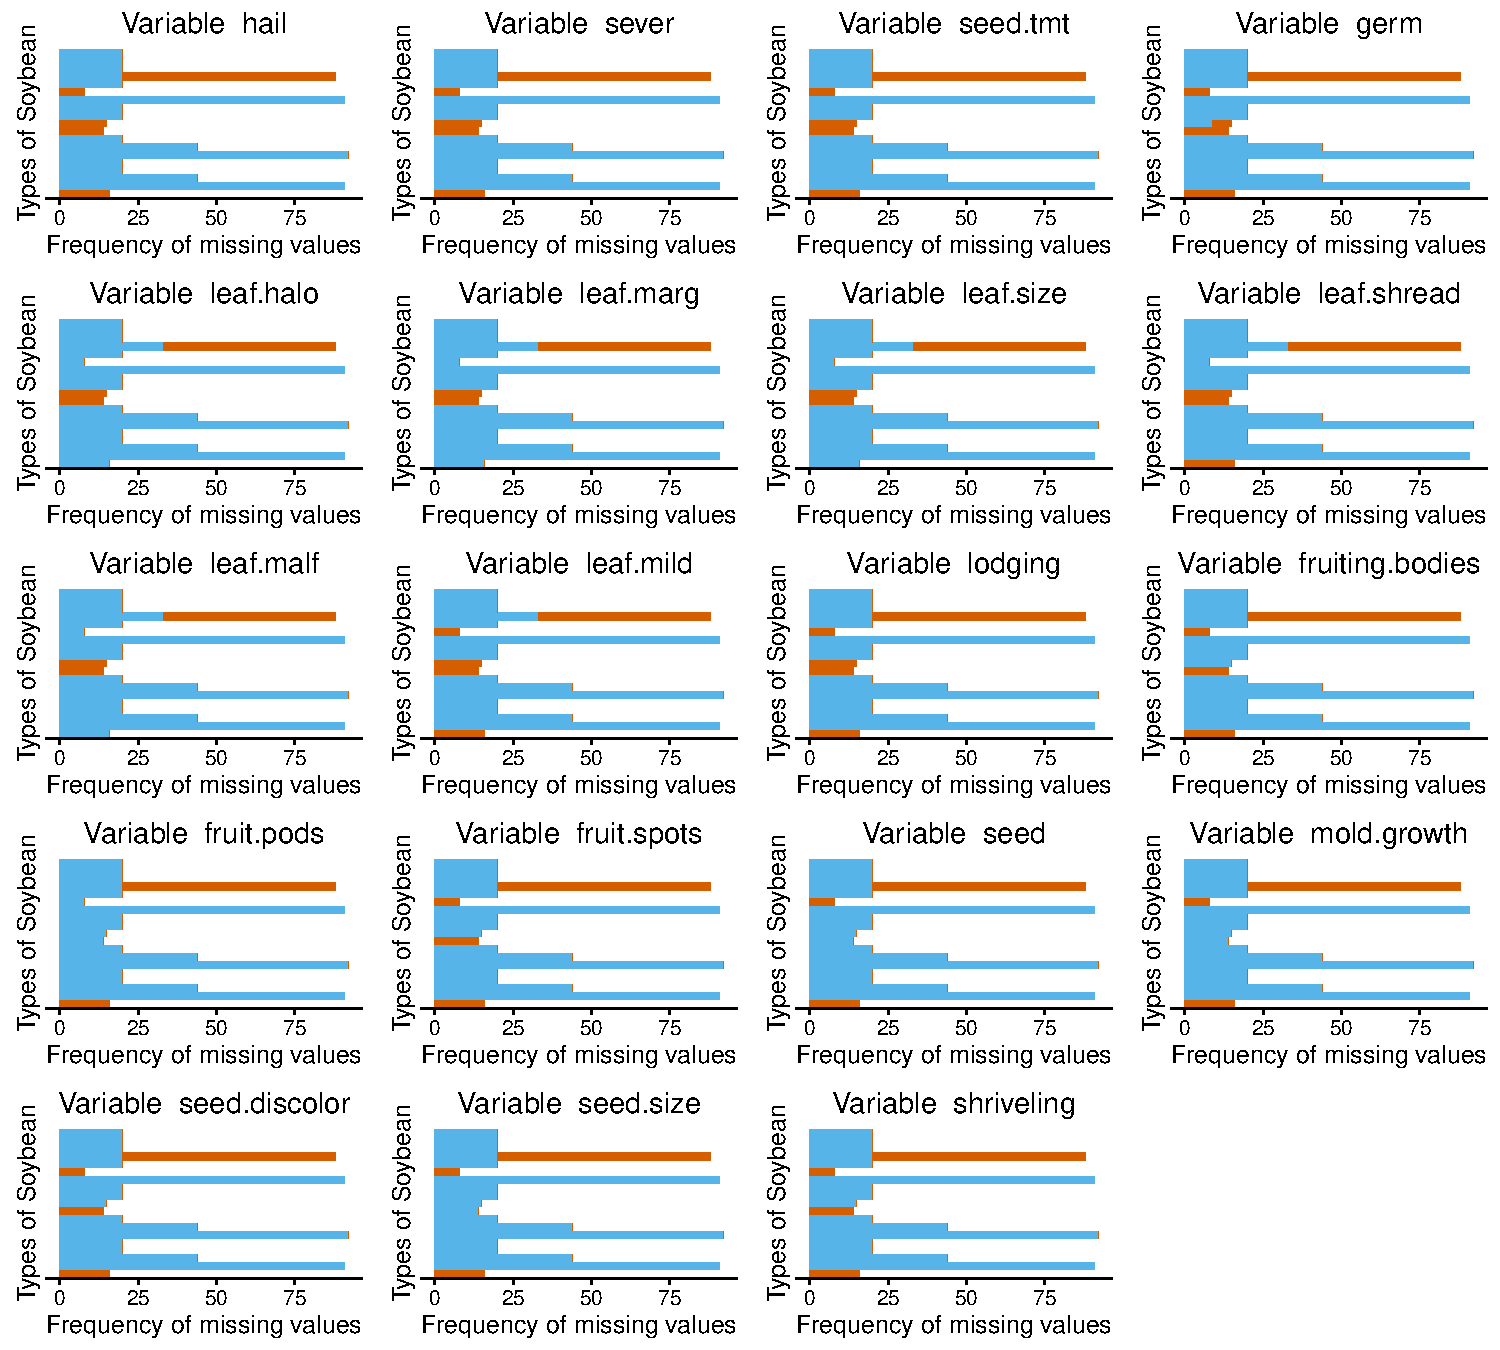
\includegraphics{hw3-012}

\item
Develop a strategy for handling missing data, either by eliminating predictors or imputation.

In this dataset, the predictors with large proportion of missing values contain informative missingness. Therefore, I'd use imputation or tree-based method.
\end{itemize}

\section{Exercise 3.3}
Chapter 5 introduces Quantitative Structure-Activity Relationship (QSAR) modeling where the characteristics of a chemical compound are used to predict other chemical properties. The caret package contains a QSAR data set from Mente and Lombardo (2005). Here, the ability of a chemical to permeate the blood-brain barrier was experimentally determined for 208 compounds. 134 descriptors were measured for each compound.
\begin{itemize}
\item
Start R and use these commands to load the data:
\begin{Schunk}
\begin{Sinput}
> library(caret)
> data(BloodBrain)
\end{Sinput}
\end{Schunk}
use ?BloodBrain to see more details
The numeric outcome is contained in the vector logBBB while the predictors
are in the data frame bbbDescr.
\item
Do any of the individual predictors have degenerate distributions?
\begin{Schunk}
\begin{Sinput}
> nearZeroVar(bbbDescr)
\end{Sinput}
\begin{Soutput}
[1]  3 16 17 22 25 50 60
\end{Soutput}
\begin{Sinput}
> length(nearZeroVar(bbbDescr))
\end{Sinput}
\begin{Soutput}
[1] 7
\end{Soutput}
\begin{Sinput}
> 
\end{Sinput}
\end{Schunk}
Yes, there are 7 predictors that have frequency ratio below 0.05.

\item
Generally speaking, are there strong relationships between the predictor
data? If so, how could correlations in the predictor set be reduced?
Does this have a dramatic effect on the number of predictors available for
modeling?
\begin{Schunk}
\begin{Sinput}
> correlation = cor(bbbDescr)
> highCorr <- findCorrelation(correlation, cutoff = .75)
> length(highCorr)
\end{Sinput}
\begin{Soutput}
[1] 66
\end{Soutput}
\begin{Sinput}
> ncol(bbbDescr)
\end{Sinput}
\begin{Soutput}
[1] 134
\end{Soutput}
\end{Schunk}
Yes, there are some that are highly correlated with each other. I can eliminate columns that are correlated with each above 0.75. This will remove 66 predictors, which amount of half the original data.
\end{itemize}
\end{document}
